\subsection{Grammar is inflexible}

One might argue that Peano's numbers are different to the tally we all use.  For example, in a tally we might 
add strokes to either side.  For instance:
\begin{center}
    \StrokeOne~\StrokeTwo = \StrokeThree = \StrokeTwo~\StrokeOne,
    i.e.\ $1+2=3=2+1$.
\end{center}
This is possible but requires a different grammar.  To make the point clear let us 
use $L$ for tallies on the left and $R$ for tallies on the right, and use a $0$ for 
the empty space.
\begin{center}
\begin{Gcode}[]
<LRNat> ::= 0
         | L <LRNat>
         | <LRNat> R
\end{Gcode}
\end{center}
If we graph some of the accepted words we see an immediate difference.
Note here we include parentheses to clarify the order in which 
words like \code{L0R} can be accepted.  Those are not part of the 
original string but indicate how the grammar sees these.
\begin{center}
    \begin{tikzpicture}[xscale=1.3]
        \node[draw] (LL0) at (-4,-2) {
            \begin{tikzpicture}[scale=0.5]
                \node[scale=0.5] (0) at (0,0) {0};
                \node[scale=0.5] (L0) at (-1,-1) {L0};
                \node[scale=0.5] (LL0) at (-2,-2) {LL0};
                \draw[-] (0) -- (L0) -- (LL0);
            \end{tikzpicture}};
        \node[draw] (RL0) at (0,2) {
            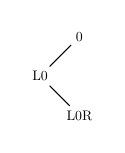
\begin{tikzpicture}[scale=0.5]
                \node[scale=0.5] (0) at (0,0) {0};
                \node[scale=0.5] (L0) at (-1,-1) {L0};
                \node[scale=0.5] (RL0) at (0,-2) {L0R};
                \draw[-] (0) -- (L0) -- (RL0);
            \end{tikzpicture}};

        \node[draw] (L0) at (-2, 0) {
            \begin{tikzpicture}[scale=0.5]
                \node[scale=0.5] (0) at (0,0) {0};
                \node[scale=0.5] (L0) at (-1,-1) {L0};
                \draw[-] (0) -- (L0);
            \end{tikzpicture}};
        \node[draw] (0) at (0,0) {0};
        \node[draw] (0Rx) at ( 2, 0) {
            \begin{tikzpicture}[scale=0.5]
                \node[scale=0.5] (0) at (0,0) {0};
                \node[scale=0.5] (0R) at ( 1,-1) {0R};
                \draw[-] (0) -- (0R);
            \end{tikzpicture}};

        \node[draw] (0RR) at ( 4, 2) {
            \begin{tikzpicture}[scale=0.5]
                \node[scale=0.5] (0) at (0,0) {0};
                \node[scale=0.5] (0R) at (1,-1) {0R};
                \node[scale=0.5] (0RR) at ( 2,-2) {0RR};
                \draw[-] (0) -- (0R) -- (0RR);
            \end{tikzpicture}};
        \node[draw] (0RL) at (0,-2) {
            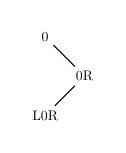
\begin{tikzpicture}[scale=0.5]
                \node[scale=0.5] (0) at (0,0) {0};
                \node[scale=0.5] (0R) at ( 1,-1) {0R};
                \node[scale=0.5] (0RL) at (0,-2) {L0R};
                \draw[-] (0) -- (0R) -- (0RL);
            \end{tikzpicture}};

        \draw[thick,->] (L0) edge["L"] (LL0);
        \draw[thick,->] (L0) edge["R"] (RL0);
        
        \draw[thick,->] (0) edge["L"] (L0);
        \draw[thick,->] (0) edge["R"] (0Rx);

        \draw[thick,->] (0Rx) edge["R"] (0RR);
        \draw[thick,->] (0Rx) edge["L"] (0RL);
    \end{tikzpicture}
\end{center}
% \begin{center}
%     \code{L0:LRNat}, \code{0R:LRNat}, and \code{L0R:LRNat}.
% \end{center}
Yet nothing in this treats \code{L0}=\code{0R}.  So left/right 
tallies are in the sense of the grammar quite different.  If we 
want to overcome this we will need to add more properties to the 
semantics (meaning) of grammar such as by adding ways rewrite.
This will come up when we later discuss relations.
